\documentclass{standalone}
\usepackage{tikz}
\usetikzlibrary{patterns, positioning}

\begin{document}
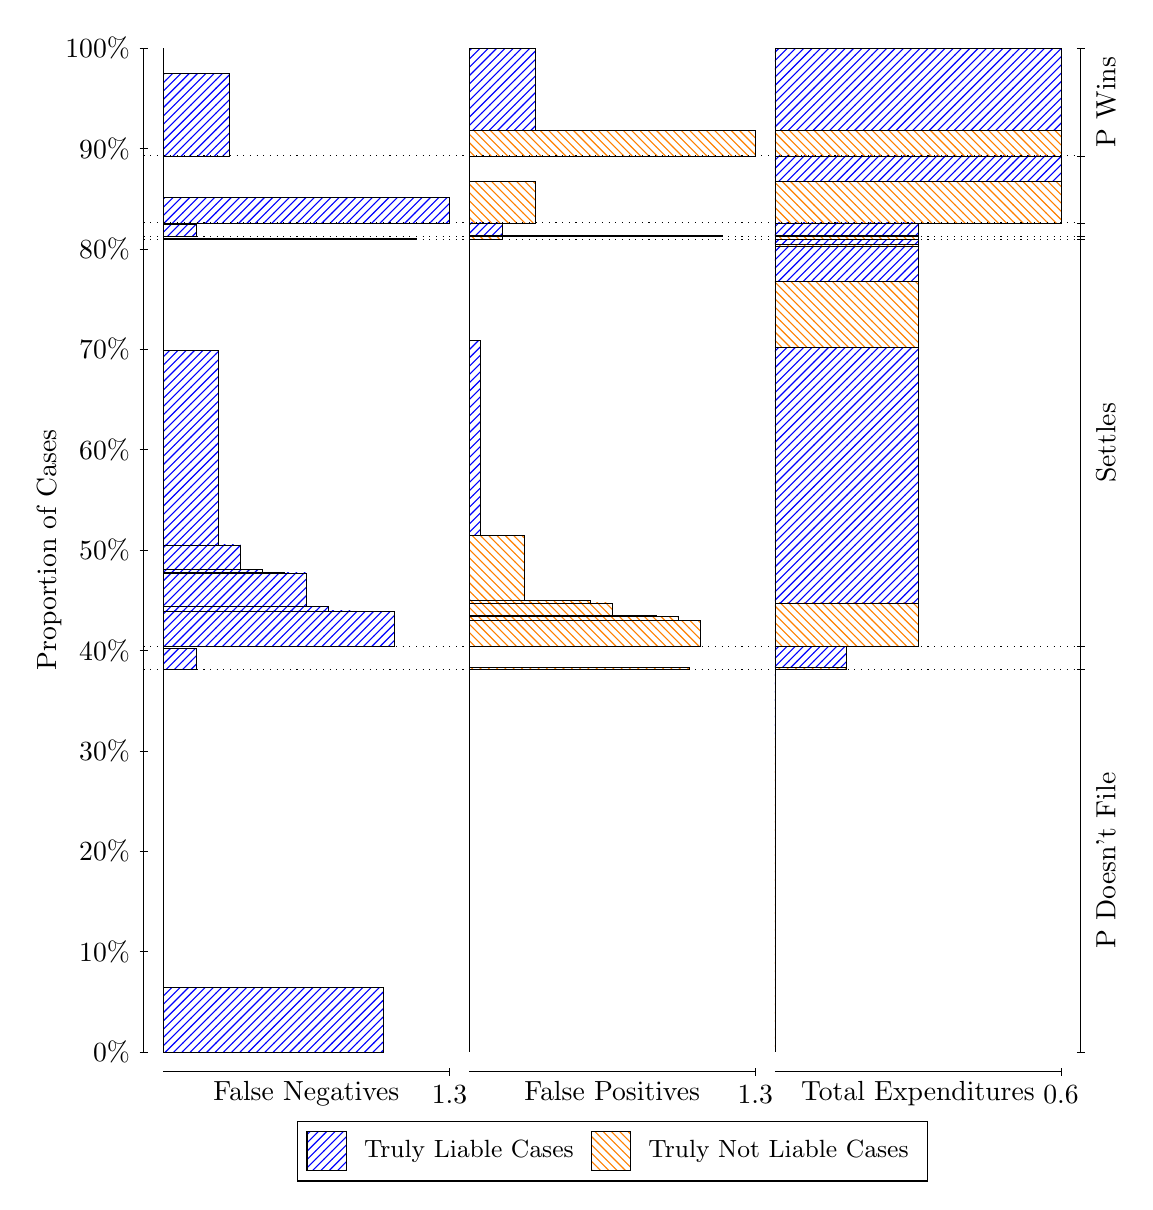
\begin{tikzpicture}
\draw[black, very thin] (1.5,1.75) -- (1.5,14.5);
\node[rotate=90, anchor=center] at (0.3, 8.125) {Proportion of Cases};
\draw[black, very thin] (1.45,1.75) -- (1.55,1.75);
\node[anchor=east] at (1.45, 1.75) {0\%};
\draw[black, very thin] (1.45,3.025) -- (1.55,3.025);
\node[anchor=east] at (1.45, 3.025) {10\%};
\draw[black, very thin] (1.45,4.3) -- (1.55,4.3);
\node[anchor=east] at (1.45, 4.3) {20\%};
\draw[black, very thin] (1.45,5.575) -- (1.55,5.575);
\node[anchor=east] at (1.45, 5.575) {30\%};
\draw[black, very thin] (1.45,6.85) -- (1.55,6.85);
\node[anchor=east] at (1.45, 6.85) {40\%};
\draw[black, very thin] (1.45,8.125) -- (1.55,8.125);
\node[anchor=east] at (1.45, 8.125) {50\%};
\draw[black, very thin] (1.45,9.4) -- (1.55,9.4);
\node[anchor=east] at (1.45, 9.4) {60\%};
\draw[black, very thin] (1.45,10.675) -- (1.55,10.675);
\node[anchor=east] at (1.45, 10.675) {70\%};
\draw[black, very thin] (1.45,11.95) -- (1.55,11.95);
\node[anchor=east] at (1.45, 11.95) {80\%};
\draw[black, very thin] (1.45,13.225) -- (1.55,13.225);
\node[anchor=east] at (1.45, 13.225) {90\%};
\draw[black, very thin] (1.45,14.5) -- (1.55,14.5);
\node[anchor=east] at (1.45, 14.5) {100\%};

\draw[black, very thin] (13.4,1.75) -- (13.4,14.5);
\draw[black, very thin] (13.35,1.75) -- (13.45,1.75);
\node[anchor=west] at (13.35, 1.75) {};
\draw[black, very thin] (13.35,6.6116) -- (13.45,6.6116);
\node[anchor=west] at (13.35, 6.6116) {};
\draw[black, very thin] (13.35,6.9006) -- (13.45,6.9006);
\node[anchor=west] at (13.35, 6.9006) {};
\draw[black, very thin] (13.35,12.071) -- (13.45,12.071);
\node[anchor=west] at (13.35, 12.071) {};
\draw[black, very thin] (13.35,12.11) -- (13.45,12.11);
\node[anchor=west] at (13.35, 12.11) {};
\draw[black, very thin] (13.35,12.28) -- (13.45,12.28);
\node[anchor=west] at (13.35, 12.28) {};
\draw[black, very thin] (13.35,13.13) -- (13.45,13.13);
\node[anchor=west] at (13.35, 13.13) {};
\draw[black, very thin] (13.35,14.5) -- (13.45,14.5);
\node[anchor=west] at (13.35, 14.5) {};

\draw[black, very thin, pattern color=blue, pattern=north east lines] (1.75,1.75) rectangle (4.5449,2.574);
\draw[black, very thin, pattern color=orange, pattern=north west lines] (1.75,2.574) rectangle (1.75,6.6116);
\draw[black, very thin, pattern color=blue, pattern=north east lines] (1.75,6.6116) rectangle (2.1692,6.8733);
\draw[black, very thin, pattern color=orange, pattern=north west lines] (1.75,6.8733) rectangle (1.75,6.9006);
\draw[black, very thin, pattern color=blue, pattern=north east lines] (1.75,6.9006) rectangle (4.6846,7.3425);
\draw[black, very thin, pattern color=blue, pattern=north east lines] (1.75,7.3425) rectangle (4.4051,7.3472);
\draw[black, very thin, pattern color=blue, pattern=north east lines] (1.75,7.3472) rectangle (4.1256,7.3519);
\draw[black, very thin, pattern color=blue, pattern=north east lines] (1.75,7.3519) rectangle (3.8462,7.4092);
\draw[black, very thin, pattern color=blue, pattern=north east lines] (1.75,7.4092) rectangle (3.5667,7.8343);
\draw[black, very thin, pattern color=blue, pattern=north east lines] (1.75,7.8343) rectangle (3.2872,7.836);
\draw[black, very thin, pattern color=blue, pattern=north east lines] (1.75,7.836) rectangle (3.0077,7.8775);
\draw[black, very thin, pattern color=blue, pattern=north east lines] (1.75,7.8775) rectangle (2.7282,8.1893);
\draw[black, very thin, pattern color=blue, pattern=north east lines] (1.75,8.1893) rectangle (2.4487,10.658);
\draw[black, very thin, pattern color=orange, pattern=north west lines] (1.75,10.658) rectangle (1.75,12.071);
\draw[black, very thin, pattern color=blue, pattern=north east lines] (1.75,12.071) rectangle (4.9641,12.078);
\draw[black, very thin, pattern color=orange, pattern=north west lines] (1.75,12.078) rectangle (1.75,12.11);
\draw[black, very thin, pattern color=blue, pattern=north east lines] (1.75,12.11) rectangle (2.1692,12.266);
\draw[black, very thin, pattern color=orange, pattern=north west lines] (1.75,12.266) rectangle (1.75,12.28);
\draw[black, very thin, pattern color=blue, pattern=north east lines] (1.75,12.28) rectangle (5.3833,12.604);
\draw[black, very thin, pattern color=orange, pattern=north west lines] (1.75,12.604) rectangle (1.75,13.13);
\draw[black, very thin, pattern color=blue, pattern=north east lines] (1.75,13.13) rectangle (2.5885,14.174);
\draw[black, very thin, pattern color=orange, pattern=north west lines] (1.75,14.174) rectangle (1.75,14.5);
\draw[black, very thin, pattern color=orange, pattern=north west lines] (5.6333,1.75) rectangle (5.6333,5.7876);
\draw[black, very thin, pattern color=blue, pattern=north east lines] (5.6333,5.7876) rectangle (5.6333,6.6116);
\draw[black, very thin, pattern color=orange, pattern=north west lines] (5.6333,6.6116) rectangle (8.4282,6.6389);
\draw[black, very thin, pattern color=blue, pattern=north east lines] (5.6333,6.6389) rectangle (5.6333,6.9006);
\draw[black, very thin, pattern color=orange, pattern=north west lines] (5.6333,6.9006) rectangle (8.5679,7.2324);
\draw[black, very thin, pattern color=orange, pattern=north west lines] (5.6333,7.2324) rectangle (8.2885,7.2848);
\draw[black, very thin, pattern color=orange, pattern=north west lines] (5.6333,7.2848) rectangle (8.009,7.294);
\draw[black, very thin, pattern color=orange, pattern=north west lines] (5.6333,7.294) rectangle (7.7295,7.2955);
\draw[black, very thin, pattern color=orange, pattern=north west lines] (5.6333,7.2955) rectangle (7.45,7.454);
\draw[black, very thin, pattern color=orange, pattern=north west lines] (5.6333,7.454) rectangle (7.1705,7.454);
\draw[black, very thin, pattern color=orange, pattern=north west lines] (5.6333,7.454) rectangle (7.1705,7.4802);
\draw[black, very thin, pattern color=orange, pattern=north west lines] (5.6333,7.4802) rectangle (6.891,7.4812);
\draw[black, very thin, pattern color=orange, pattern=north west lines] (5.6333,7.4812) rectangle (6.6115,7.4822);
\draw[black, very thin, pattern color=orange, pattern=north west lines] (5.6333,7.4822) rectangle (6.3321,8.3137);
\draw[black, very thin, pattern color=blue, pattern=north east lines] (5.6333,8.3137) rectangle (5.7731,10.783);
\draw[black, very thin, pattern color=blue, pattern=north east lines] (5.6333,10.783) rectangle (5.6333,12.071);
\draw[black, very thin, pattern color=orange, pattern=north west lines] (5.6333,12.071) rectangle (6.0526,12.103);
\draw[black, very thin, pattern color=blue, pattern=north east lines] (5.6333,12.103) rectangle (5.6333,12.11);
\draw[black, very thin, pattern color=orange, pattern=north west lines] (5.6333,12.11) rectangle (8.8474,12.124);
\draw[black, very thin, pattern color=blue, pattern=north east lines] (5.6333,12.124) rectangle (6.0526,12.28);
\draw[black, very thin, pattern color=orange, pattern=north west lines] (5.6333,12.28) rectangle (6.4718,12.806);
\draw[black, very thin, pattern color=blue, pattern=north east lines] (5.6333,12.806) rectangle (5.6333,13.13);
\draw[black, very thin, pattern color=orange, pattern=north west lines] (5.6333,13.13) rectangle (9.2667,13.455);
\draw[black, very thin, pattern color=blue, pattern=north east lines] (5.6333,13.455) rectangle (6.4718,14.5);
\draw[black, very thin, pattern color=orange, pattern=north west lines] (9.5167,1.75) rectangle (9.5167,5.7876);
\draw[black, very thin, pattern color=blue, pattern=north east lines] (9.5167,5.7876) rectangle (9.5167,6.6116);
\draw[black, very thin, pattern color=orange, pattern=north west lines] (9.5167,6.6116) rectangle (10.425,6.6389);
\draw[black, very thin, pattern color=blue, pattern=north east lines] (9.5167,6.6389) rectangle (10.425,6.9006);
\draw[black, very thin, pattern color=orange, pattern=north west lines] (9.5167,6.9006) rectangle (11.333,7.454);
\draw[black, very thin, pattern color=blue, pattern=north east lines] (9.5167,7.454) rectangle (11.333,10.703);
\draw[black, very thin, pattern color=orange, pattern=north west lines] (9.5167,10.703) rectangle (11.333,11.534);
\draw[black, very thin, pattern color=blue, pattern=north east lines] (9.5167,11.534) rectangle (11.333,11.976);
\draw[black, very thin, pattern color=orange, pattern=north west lines] (9.5167,11.976) rectangle (11.333,12.005);
\draw[black, very thin, pattern color=blue, pattern=north east lines] (9.5167,12.005) rectangle (11.333,12.071);
\draw[black, very thin, pattern color=orange, pattern=north west lines] (9.5167,12.071) rectangle (11.333,12.103);
\draw[black, very thin, pattern color=blue, pattern=north east lines] (9.5167,12.103) rectangle (11.333,12.11);
\draw[black, very thin, pattern color=orange, pattern=north west lines] (9.5167,12.11) rectangle (11.333,12.124);
\draw[black, very thin, pattern color=blue, pattern=north east lines] (9.5167,12.124) rectangle (11.333,12.28);
\draw[black, very thin, pattern color=orange, pattern=north west lines] (9.5167,12.28) rectangle (13.15,12.806);
\draw[black, very thin, pattern color=blue, pattern=north east lines] (9.5167,12.806) rectangle (13.15,13.13);
\draw[black, very thin, pattern color=orange, pattern=north west lines] (9.5167,13.13) rectangle (13.15,13.455);
\draw[black, very thin, pattern color=blue, pattern=north east lines] (9.5167,13.455) rectangle (13.15,14.5);
\draw[black, dotted] (1.5,6.6116) -- (13.4,6.6116);
\draw[black, dotted] (1.5,6.9006) -- (13.4,6.9006);
\draw[black, dotted] (1.5,12.071) -- (13.4,12.071);
\draw[black, dotted] (1.5,12.11) -- (13.4,12.11);
\draw[black, dotted] (1.5,12.28) -- (13.4,12.28);
\draw[black, dotted] (1.5,13.13) -- (13.4,13.13);
\draw[black, very thin] (1.75,1.5) -- (5.3833,1.5);
\node[anchor=north] at (3.5667, 1.5) {False Negatives};
\draw[black, very thin] (5.3833,1.45) -- (5.3833,1.55);
\node[anchor=north] at (5.3833, 1.45) {1.3};

\draw[black, very thin] (5.6333,1.5) -- (9.2667,1.5);
\node[anchor=north] at (7.45, 1.5) {False Positives};
\draw[black, very thin] (9.2667,1.45) -- (9.2667,1.55);
\node[anchor=north] at (9.2667, 1.45) {1.3};

\draw[black, very thin] (9.5167,1.5) -- (13.15,1.5);
\node[anchor=north] at (11.333, 1.5) {Total Expenditures};
\draw[black, very thin] (13.15,1.45) -- (13.15,1.55);
\node[anchor=north] at (13.15, 1.45) {0.6};

\node[black, centered, rotate=90] at (13.72, 4.1808) {P Doesn't File};

\node[black, centered, rotate=90] at (13.72, 9.486) {Settles};



\node[black, centered, rotate=90] at (13.72, 13.815) {P Wins};

\draw (7.449999999999999,1.5) node[draw=none] (baseCoordinate) {};
\begin{scope}[align=center]
        \matrix[scale=0.5, draw=black, below=0.5cm of baseCoordinate, nodes={draw}, column sep=0.1cm]{
            \node[rectangle, draw, minimum width=0.5cm, minimum height=0.5cm, pattern=north east lines, pattern color=blue] {}; &
            \node[draw=none, font=\small] (B) {Truly Liable Cases}; &
            \node[rectangle, draw, minimum width=0.5cm, minimum height=0.5cm, pattern=north west lines, pattern color=orange] {}; &
            \node[draw=none, font=\small] (B) {Truly Not Liable Cases}; \\
            };
\end{scope}

\end{tikzpicture}
\end{document}